\chapter{A First Example}
We will now look at a simple example that demonstrates all the features of
Bayesian statistics. The problem is quite simple, but we will be able to see
how we start with some probabilities at the beginning of the problem (these are
called {\it prior probabilities}), and how exactly these get updated
into after we get more information (these updated probabilities are called
{\it posterior probabilities}). To help make things clear (hopefully), we will
use a table that we will call a {\it Bayes Box} to help us calculate the
posterior probabilities.

Here we will study a simple example to see what is going on with Bayesian
statistics. Suppose that there are two balls in a bag. We know in advance
that at least one of them is black. But we're not sure whether they're both
black, or whether one is black and one is white. To keep things concise, we
should label our two competing hypotheses. We could call them whatever we want,
but I will call them \bw~and \bb. So, at the beginning of the problem, we know
that one and only one of the following statements/hypothesis is true:\\

\begin{center}
\begin{tabular}{|l|}
\hline
\bb: Both balls are black\\
\bw: One ball is black and the other is white.\\
\hline
\end{tabular}
\end{center}
We will do an experiment to help us determine which of these two hypotheses is
true. The experiment is to reach into the bag, pull out one of the balls, and
observe its colour. {\it The result of this experiment is that the observed
ball was black}. We will now do a Bayesian analysis of this result, to see how
it works.

\section{Bayes' Box}
A Bayesian analysis starts by choosing some values for the prior probabilities.
We have our two competing hypotheses \bw~and \bb, and we need to choose some
probability values to describe how sure we are that each of these is true.
For simplicity, we will assume that we don't have much of an idea which is true,
and so we will use the following prior probabilities.
\begin{eqnarray}
P(\bb) &=& 0.5\\
P(\bw) &=& 0.5.
\end{eqnarray}
This describes the fact that before we did the experiment, we were very
uncertain about which of the two hypotheses was true. Note that \bw~and \bb~are
{\it mutually exclusive}. That means that only one of
them can be true, they can't both be true (that would be contradictory). We will
usually use mutually exclusive hypotheses in this course. They are also
{\it exhaustive}, which means that we assume the true solution is contained
in the set of hypothesis that we consider. We will also assume this every time.

I will now present a Bayes' box, which lists all the hypotheses (in this case
two) that might be true, and the prior probabilities. There are some extra
columns which we haven't discussed yet, which will be needed in order to
figure out the posterior probabilities in the final column.
\begin{table}[h!]
\begin{center}
\begin{tabular}{|c|c|c|c|c|}
\hline
{\bf Hypotheses} & {\tt prior} & {\tt likelihood} &
{\tt prior $\times$ likelihood} & {\tt posterior}\\
\hline
{\tt BB} & 0.5 &   &  & \\
{\tt BW} & 0.5 &   &  & \\
\hline
Totals: & 1 & & & \\
\hline
\end{tabular}
\end{center}
\end{table}
The first column of a Bayes' Box is just the list of hypotheses we are
considering. If you are to construct a Bayes' box for a new problem, just think
about what the possible answers to the problem are, and list them in the first
column. The second column lists the prior probabilities for each of the
hypotheses.
Since we know one and only
one of the two hypotheses is true, and we want our prior probabilities to
describe a large amount of uncertainty, we shall say that there is a 50\%
probability that \bb~is true and a 50\% probability that \bw~is true.
The prior column should always sum to 1. Remember, the prior probabilities
only describe our initial uncertainty, before taking into account the
data. Hopefully the data will help by changing these probabilities to
something else!

\subsection{Likelihood}
The third column is called {\it likelihood}, and this is a really important
column. It is a quantity that will be used for calculating the posterior
probabilities. In colloquial language, likelihood is synonymous with
probability; it means the same thing. In statistics, likelihood is a very
specific kind of probability. If you consider each of the 


If you have taken STATS 210 and used the maximum likelihood method, where you
find the value of a parameter that maximises the likelihood function, that is
the same as the likelihood we use in this course! So you have a head start
in understanding this concept.

\subsection{Finding the Likelihood Values}

\section{Bayes' Rule}
Bayes' rule is an equation from probability theory, shown in
Figure~\ref{fig:bayes_neon}.

\begin{figure}
\begin{center}
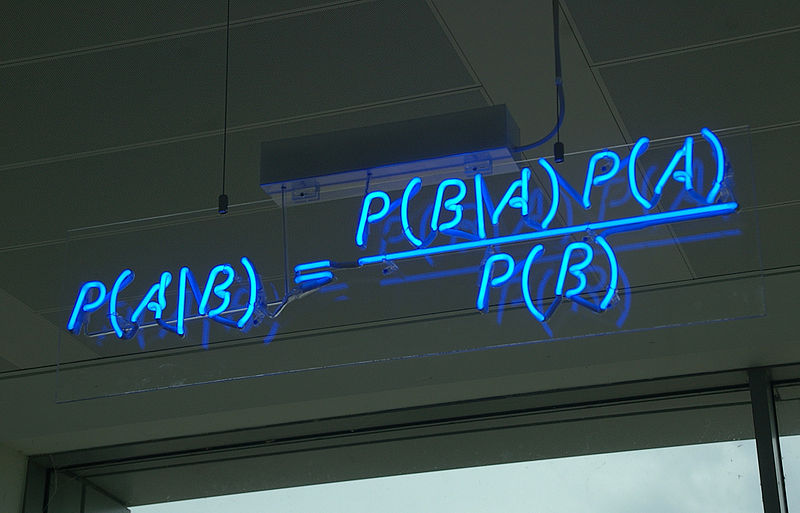
\includegraphics[scale=0.4]{bayes_neon.jpg}
\caption{A blue neon sign displaying Bayes' rule.
You can use it to calculate the probability of $A$ {\it given} $B$,
if you know the values of some other probabilities on the right hand side.
Image credit: Matt Buck. Obtained from Wikimedia Commons.
\label{fig:bayes_neon}}
\end{center}
\end{figure}

The 

In the above section, we did some calculations to work out the numbers in the
Bayes' Box, particularly the posterior probabilities, which are the ultimate
goal of the calculation. {\it What we were actually doing in these calculations
was applying Bayes' rule}. We actually applied Bayes' rule twice, once to
compute $P(\bb | D)$ and once to calculate $P(\bw | D)$.


\begin{center}
\begin{tabular}{|c|}
\hline
{\bf When you use a Bayes' Box to calculate posterior probabilities,}\\
{\bf you are really just applying Bayes' rule a lot of times:}\\
{\bf once for each row of the Bayes' Box.}\\
\hline
\end{tabular}
\end{center}





In general, Bayes' rule looks like this:
\begin{eqnarray}
P(H|D) = \frac{P(H)P(D|H)}{P(D)}
\end{eqnarray}
Here's what all the terms mean:
\begin{itemize}
\item $P(H|D)$ is the {\bf posterior probability}. It describes how sure we are that
hypothesis $H$ is true, given that we have observed data $D$. Calculating
posterior probabilities is the main goal of Bayesian statistics!
\item $P(H)$ is the {\bf prior probability}, which describes how sure we were that
$H$ was true, before we observed the data $D$.
\item $P(D|H)$ is the {\bf likelihood}. If you were to assume that $H$ is true,
this is the probability that you would have observed data $D$.
\item $P(D)$ is the {\bf marginal likelihood}. This is the probability that you
would have observed data $D$, {\it whether $H$ is true or not}.
\end{itemize}










\section{Phone Example}
This example appeared in the 2012 final exam.


